\documentclass{article}
% translate with >> pdflatex -shell-escape <file>

% This file is an extract of the PGFPLOTS manual, copyright by Christian Feuersaenger.
% 
% Feel free to use it as long as you cite the pgfplots manual properly.
%
% See
%   http://pgfplots.sourceforge.net/pgfplots.pdf
% for the complete manual.
%
% Any required input files (for <plot table> or <plot file> or the table package) can be downloaded
% at
% http://www.ctan.org/tex-archive/graphics/pgf/contrib/pgfplots/doc/latex/
% and
% http://www.ctan.org/tex-archive/graphics/pgf/contrib/pgfplots/doc/latex/plotdata/
\usepackage{ae,aecompl}
\usepackage[T1]{fontenc}
\usepackage[utf8]{inputenc}
\usepackage{textcomp}


\usepackage{pgfplots}
\pgfplotsset{compat=newest}

\pagestyle{empty}

\usepgfplotslibrary{ternary}

\begin{document}


\section{Bevezetés}
A háromkomponensű vagy terner rendszerek nem csak elméleti szempontból vetnek fel érdekes kérdéseket, de nagy gyakorlati jelentõségük is van, például a kohászatban, műanyagiparban.
Gondoljunk az olvadékokra, ötvözetekre, melyekben egy vagy több szilárd fázis tarthat egyensúlyt egy vagy két közös anyagot tartalmazó folyadékfázissal, vagy a polimerek oldására stb.
A terner rendszerekben a komponensek egymásban való kölcsönös oldhatósága különböző.
Minden ilyen rendszernél található olyan nyomás és/vagy hőmérséklet tartomány, melynél legalább két összetevő csak korlátosan elegyedik.
A harmadik komponens jelenléte - amennyiben ez részben vagy teljesen elegyedik a két másik komponenssel - megváltoztatja a két részben elegyedõ komponens kölcsönös oldhatóságát.

A terner rendszerek állapotának leírásához a nyomáson és hőmérsékleten kívül az összetételre van szükség, amennyiben a rendszerben kémiai reakció nem játszódik le.
Minthogy két komponens móltörtjének ismeretében a harmadik komponens móltörtje kiszámítható, ezért a szabadsági fokok száma egy ilyen rendszerben 4.
Adott hőmérsékleten és nyomáson tehát a rendszer állapotát a 2 összetétel adat egyértelműen meghatározza.
Ahhoz, hogy egy terner rendszer fázisdiagramját síkban ábrázolhassuk, két paramétert - célszerûen a nyomást és hőmérsékletet - állandónak kell vennünk.
Ez esetben a három komponens által meghatározott összetételt egyenlő oldalú háromszögben tüntethetjük fel.
A háromszög csúcsai jelentik a tiszta komponensekből álló egykomponensű rendszereket.
A könnyebb átláthatóságért célszerű a háromszögre egy körüljárási irányt meghatározni, amely a mi esetünkben az óramutató járásával ellentétes lesz. A háromszög oldalain az egyes komponensek móltörtjét - vagy tömegszázalékátszokás feltüntetni (\ref{fig:ccw}. ábra).

\begin{figure}
\centering
\begin{tikzpicture}
\begin{ternaryaxis}[
	xlabel=ecetsav m\%,
	ylabel=víz m\%,
	zlabel=kloroform m\%,
	minor tick num=9,
	grid=both,
	axis on top,
	xmin=0,
	xmax=100,
	ymin=0,
	ymax=100,
	zmin=0,
	zmax=100,
]
% plotdata/ternary_data.txt is a table of the form
%A_propene A_water A_IPA  B_propene B_water B_IPA
% 0.0009   0.9990  0      0.9333    0.0667  0
% 0.0009   0.9988  0.0002 0.9303    0.0665  0.0032
% 0.0011   0.9975  0.0013 0.9135    0.0673  0.0191
% 0.0013   0.9962  0.0024 0.8956    0.0693  0.0351
%...
	\addplot3[
		point meta=rand,
		tieline={
			each nth tie=8,
			tieline style={contour prepared}
		},
		fill=blue!10,
	]
	table [x=A_IPA,y=A_water,z=A_propene] 
		{plotdata/ternary_data.txt};
	\draw [decorate, decoration={brace,amplitude=15pt,raise=1pt}] (0,100) -- (50,0)  node [midway, xshift=-1mm, auto, swap, outer sep=10pt,font=\tiny]{debtee};
	\draw (0,100) -- (10,50)  node [midway, xshift=-1mm, auto, swap, outer sep=10pt,font=\tiny]{debtee};

\end{ternaryaxis}
\end{tikzpicture}
\caption{Terner rendszer diagramja.}
\label{fig:ccw}
\end{figure}

\newpage
\newpage
\begin{figure}
\centering
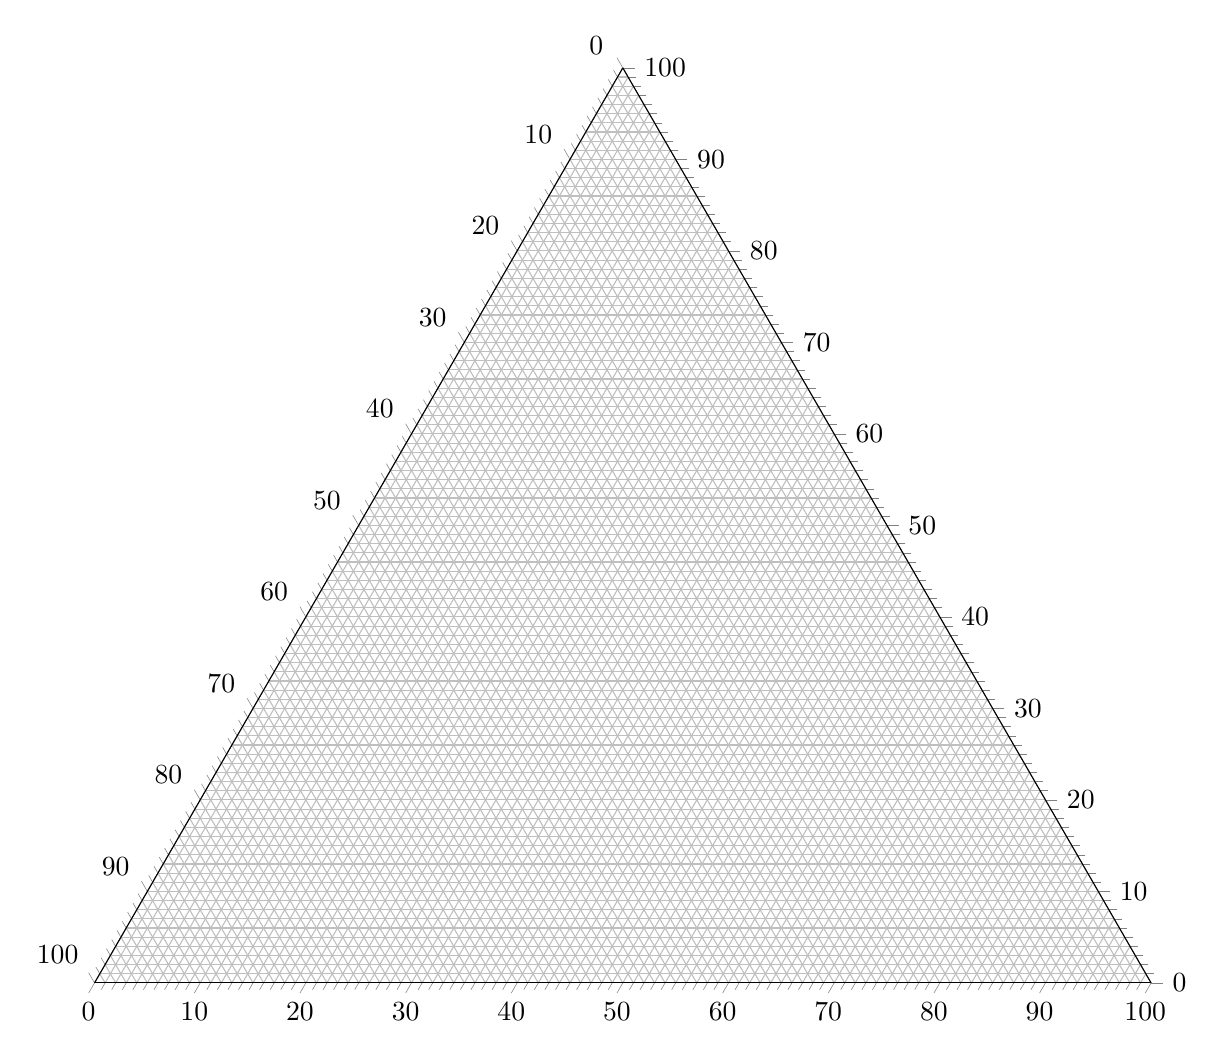
\begin{tikzpicture}
\begin{ternaryaxis}[minor tick num=9,grid=both,axis on top,xmin=0,xmax=100,ymin=0,ymax=100,zmin=0,zmax=100,width=15cm,height=15cm,]
% plotdata/ternary_data.txt is a table of the form
%A_propene A_water A_IPA  B_propene B_water B_IPA
% 0.0009   0.9990  0      0.9333    0.0667  0
% 0.0009   0.9988  0.0002 0.9303    0.0665  0.0032
% 0.0011   0.9975  0.0013 0.9135    0.0673  0.0191
% 0.0013   0.9962  0.0024 0.8956    0.0693  0.0351
%...
\end{ternaryaxis}
\end{tikzpicture}
%\caption{Terner diagram..}
\label{fig:ccw}
\end{figure}



\end{document}
